%% ============================================================================
%% Frontiers in Digital Health - Manuscript (FULLY REVISED - ALL REFERENCES)
%% Title: Machine Learning-Driven Prediction of Emergency Department Length of 
%%        Stay, Admission, and Hospitalization Using Data Available at Triage
%% ============================================================================

\documentclass[harvard,article]{frontiersinFPHY_FAMS}

\usepackage{url,lineno,amsmath,amssymb,graphicx}
\usepackage{booktabs,multirow,tabularx,caption,subcaption,float}
\usepackage{array}
\usepackage[colorlinks=true, urlcolor=blue, citecolor=black, linkcolor=black]{hyperref}

\linenumbers
\onecolumn

\def\keyFont{\fontsize{8}{11}{\helveticabold}}
\def\firstAuthorLast{Onwurah {et~al.}}

\title{Machine Learning-Driven Prediction of Emergency Department Length of Stay, Admission, and Hospitalization Using Data Available at Triage}

\author{Onyedikachi I. Onwurah$^{1}$, Sol Richardson$^{1}$, Sheng Wu$^{2}$, and Tong Xia$^{1,*}$ \\
\vspace{0.2cm}
\small{$^{1}$Vanke School of Public Health, Tsinghua University, Beijing, China}\\
\small{$^{2}$Beijing Tsinghua Changgung Hospital, Beijing, China} \\
}
\correspondance{Tong Xia$^{1,*}$: tongxia@mail.tsinghua.edu.cn}

\begin{document}

\maketitle

% ============================================================================
% ABSTRACT
% ============================================================================
\begin{abstract}

\noindent\textbf{Background:} Emergency Department (ED) crowding is a critical public health challenge. Prolonged ED length of stay ($\geq$8 hours) affects over 20\% of visits. Hospital admission and prolonged hospitalization ($>$7 days) consume disproportionate resources. Clinicians currently rely on triage scales like the Emergency Severity Index (ESI), which have limited predictive accuracy. Machine learning (ML) using data available at triage could support these decisions, but evidence on model accuracy remains limited.

\noindent\textbf{Methods:} Using the MC-MED dataset (118,385 adult ED visits), we evaluated four ML models (XGBoost, LightGBM, Random Forest, TabNet) on three binary classification tasks using 29 variables available at or before the time of triage to predict: (1) prolonged ED length of stay (ED-LOS $\geq$8 hours vs. $<$8 hours), (2) hospital admission (admit vs. discharge), and (3) prolonged hospital length of stay (hospital LOS $>$7 days vs. $\leq$7 days) among admitted patients. Area under the receiver operating characteristic curve (AUC-ROC) was the primary performance metric. SHAP (SHapley Additive exPlanations) analysis identified the most important features for each prediction task. Decision curve analysis (DCA) evaluated clinical utility.

\noindent\textbf{Results:} For ED-LOS $\geq$8 hours, Random Forest achieved the highest AUC-ROC of 0.660 (95\% CI: 0.649--0.671). For hospital admission, XGBoost achieved an AUC-ROC of 0.816 (95\% CI: 0.809--0.824), substantially outperforming the ESI baseline (AUC 0.505, 95\% CI: 0.492--0.518). For hospital LOS $>$7 days among admitted patients, Random Forest achieved an AUC-ROC of 0.670 (95\% CI: 0.662--0.680) \cite{bacchi2022}. SHAP analysis identified consistent top predictors across tasks: triage acuity level, emergency medical services (EMS) arrival, age, disease condition count, and the Charlson Comorbidity Index. Calibration analysis revealed systematic miscalibration requiring probability recalibration before clinical deployment.

\noindent\textbf{Conclusion:} ML using data at or before the time of triage shows strong discrimination for hospital admission and modest discrimination for predicting ED-LOS and prolonged hospital LOS. SHAP analysis provides interpretable feature importance to support clinical decision-making. Decision curve analysis demonstrated strong clinical utility for hospital admission prediction and modest utility for ED-LOS and hospital LOS prediction. External validation and probability recalibration are required before clinical deployment.

\noindent\textbf{Keywords:} machine learning, emergency department, hospital admission, length of stay, Shapley Additive Explanations, decision curve analysis

\end{abstract}

% ============================================================================
% INTRODUCTION
% ============================================================================
\section{INTRODUCTION}

Emergency departments (EDs) offer a fundamental service, providing emergency treatments 24 hours a day, 365 days a year, therefore representing a critical public health service role \cite{higginson2012, trzeciak2003, ricciardi2024}. Crowding in EDs has been recognised as a critical challenge in hospital administration \cite{asplin2003, rcem2025}. ED crowding has been linked to increased costs, longer waiting times, higher mortality rates, and adverse outcomes for vulnerable populations \cite{sun2013, burke2020, obermeyer2019}.

Emergency department length of stay (ED-LOS) is a significant indicator of ED bottlenecks. ED-LOS is defined as the interval from ED arrival to ED departure \cite{stone2022, ricciardi2024}. A prolonged ED-LOS is a consequence of crowding and has been associated with a 37\% elevated mortality risk among admitted patients \cite{sun2013}. Several studies have defined an extended ED-LOS as more than 3 hours \cite{ricciardi2024}, while others use thresholds of 4 to 12 hours \cite{farimani2024}. The ED-LOS threshold of 8 hours was selected for this study based on evidence linking prolonged ED boarding beyond 6-8 hours to elevated mortality \cite{sun2013} and its widespread use as a standard crowding benchmark by the American College of Emergency Physicians. Prolonged ED length of stay not only affects patient outcomes but also contributes to ambulance diversion, treatment delays for time-sensitive conditions, and inefficient resource utilization across the hospital system.

Clinicians currently rely on triage scales such as the Emergency Severity Index (ESI) to prioritize patients and predict clinical trajectories. However, the ESI demonstrates limited predictive accuracy for key outcomes such as hospital admission and prolonged length of stay when used in isolation, with AUC-ROC values typically below 0.70 \cite{levin2020}. This limitation creates an opportunity for data-driven approaches that integrate multiple patient characteristics available at triage.

Machine learning (ML) techniques are frequently used in healthcare for diagnosis, forecasting patient outcomes, and resource allocation \cite{kareemi2020, raita2019, taylor2020}. Following this approach, various studies have examined ways to predict ED-LOS, hospital admission, and hospital LOS using ML strategies \cite{wu2025, fenn2021, lin2024, wu2023}. Ricciardi et al. \cite{ricciardi2024} achieved 74.8\% accuracy for predicting ED-LOS greater than 3 hours using Random Forest. Wu et al. \cite{wu2025} found that LightGBM outperformed other models for continuous ED-LOS prediction in a Chinese hospital setting.

Shbool et al. \cite{shbool2023} applied machine learning algorithms including Random Forest and Decision Trees to predict ED length of stay, achieving an accuracy of 72.8\% using 15 triage variables on a dataset of 10,241 ED visits. They identified age, triage category, and mode of arrival as the most important predictors. Hong et al. \cite{hong2018} demonstrated that machine learning models using triage data, demographics, and patient history can predict hospital admission with AUC up to 0.88 using gradient boosting. Their study of ED visits showed that the ESI alone had limited predictive power (AUC 0.68), but machine learning models incorporating additional triage variables significantly improved performance.

However, existing models have three critical limitations. First, most studies predict ED-LOS, hospital admission, or hospital LOS in isolation, despite their clinical interdependence in real-world emergency care pathways \cite{stone2022}. Second, many models incorporate laboratory results or specialist consultations that are unavailable at triage, limiting real-time clinical applicability \cite{levin2020, xiao2023}. Third, while SHAP has been applied to individual ED prediction tasks, its systematic application across multiple cascading outcomes (ED-LOS, admission, and hospital LOS) using a unified triage-time feature set has not been explored. Additionally, decision curve analysis to evaluate clinical utility has been underutilized in this context.

Given these considerations, this work aims to build a predictive model to forecast three binary treatment outcomes using only variables available at or before triage: (1) prolonged ED-LOS ($\geq$8 hours), (2) hospital admission, and (3) prolonged hospital LOS ($>$7 days) among admitted patients.

Using the MC-MED dataset (118,385 adult ED visits from Stanford Health Care, 2020 to 2022), we evaluated four ML algorithms (XGBoost, LightGBM, Random Forest, and TabNet) on three binary classification tasks using 29 variables available at or before triage time. Predicting these outcomes in advance would be beneficial for planning staff allocation and bed management with the goal of reducing ED crowding \cite{moreno2024, canellas2024}.

% ============================================================================
% METHODS
% ============================================================================
\section{METHODS}

\subsection{Prediction Tasks}

Three binary classification tasks were formulated using only variables available at or before triage time. Task 1 predicted prolonged emergency department length of stay defined as eight hours or more versus less than eight hours \cite{sun2013, farimani2024}. The ED-LOS threshold of 8 hours was selected based on evidence linking prolonged ED boarding beyond this duration to elevated mortality \cite{sun2013} and its established use as a policy-relevant crowding benchmark in the emergency medicine literature \cite{boyle2012, morley2018}. Intermediate cutoffs (e.g., 6 or 10 hours) were not evaluated in a post-hoc sensitivity analysis, as the 8-hour threshold was chosen a priori to align directly with this operational benchmark and to preserve comparability with prior health-systems literature using the same cutoff.

Task 2 predicted hospital admission, where admission was defined as any non-discharge disposition, including inpatient, observation, and intensive care unit admissions. Discharge to home, transfer to another facility, death in the ED, hospice discharge, and leaving against medical advice (LAMA) were all classified as non-admission (discharge) outcomes \cite{kansal2025, fenn2021}.

Task 3 predicted prolonged hospital length of stay defined as more than seven days versus seven days or less, applied exclusively to admitted patients \cite{stone2022, gokhale2023}. The hospital LOS threshold of 7 days was chosen to identify patients with complex inpatient courses that disproportionately strain hospital bed capacity, consistent with prior systematic reviews of LOS prediction thresholds \cite{gokhale2023, stone2022}. As with the ED-LOS threshold, this cutoff was fixed a priori based on its clinical and operational relevance for discharge planning and bed management, rather than selected post hoc; alternative cutoffs (e.g., 5 or 10 days) were therefore not separately tested.

ED-LOS was calculated as the interval (in hours) from ED Arrival\_time to Departure\_time from the emergency department. Hospital LOS was calculated as the interval (in days) from hospital admission time (Admit\_time) to hospital discharge time, among admitted patients only. Patients with missing Admit\_time or discharge timestamps were excluded from Task 3 via listwise deletion.

\subsection{Data Resource and Preprocessing}

This study analysed the MC-MED dataset \cite{kansal2025, kansal2025b}, which contains 118,385 adult emergency department visits from Stanford Health Care between January 2020 and December 2022. The dataset includes demographics, triage vital signs, chief complaints, comorbidity measures, home medications, and visit outcomes \cite{goldberger2000}.

Figure~\ref{fig:pipeline} shows the data preprocessing pipeline. The pipeline consisted of five sequential stages. Stage one involved raw data loading from the three source tables provided with the MC-MED dataset: \texttt{visits.csv}, \texttt{meds.csv}, and \texttt{pmh.csv}. These tables were merged using the Contact Serial Number to link visit specific records and the Medical Record Number (MRN) to aggregate longitudinal medication and past medical history data. Stage two applied the chronological split into training, validation, and test sets using the pre-defined split files provided with MC-MED, which ensured temporal separation between periods with no patient appearing in more than one split. Stage three handled missing data using the procedures described in detail below. Stage four performed outcome separation, where all time dependent columns including emergency department length of stay, hospital length of stay, disposition status, arrival time, admit time, discharge time, and departure time were removed from the feature set before model training to prevent temporal and data leakage. Stage five defined the three binary classification targets as described in the preceding subsection.

\begin{figure}[t]
\centering
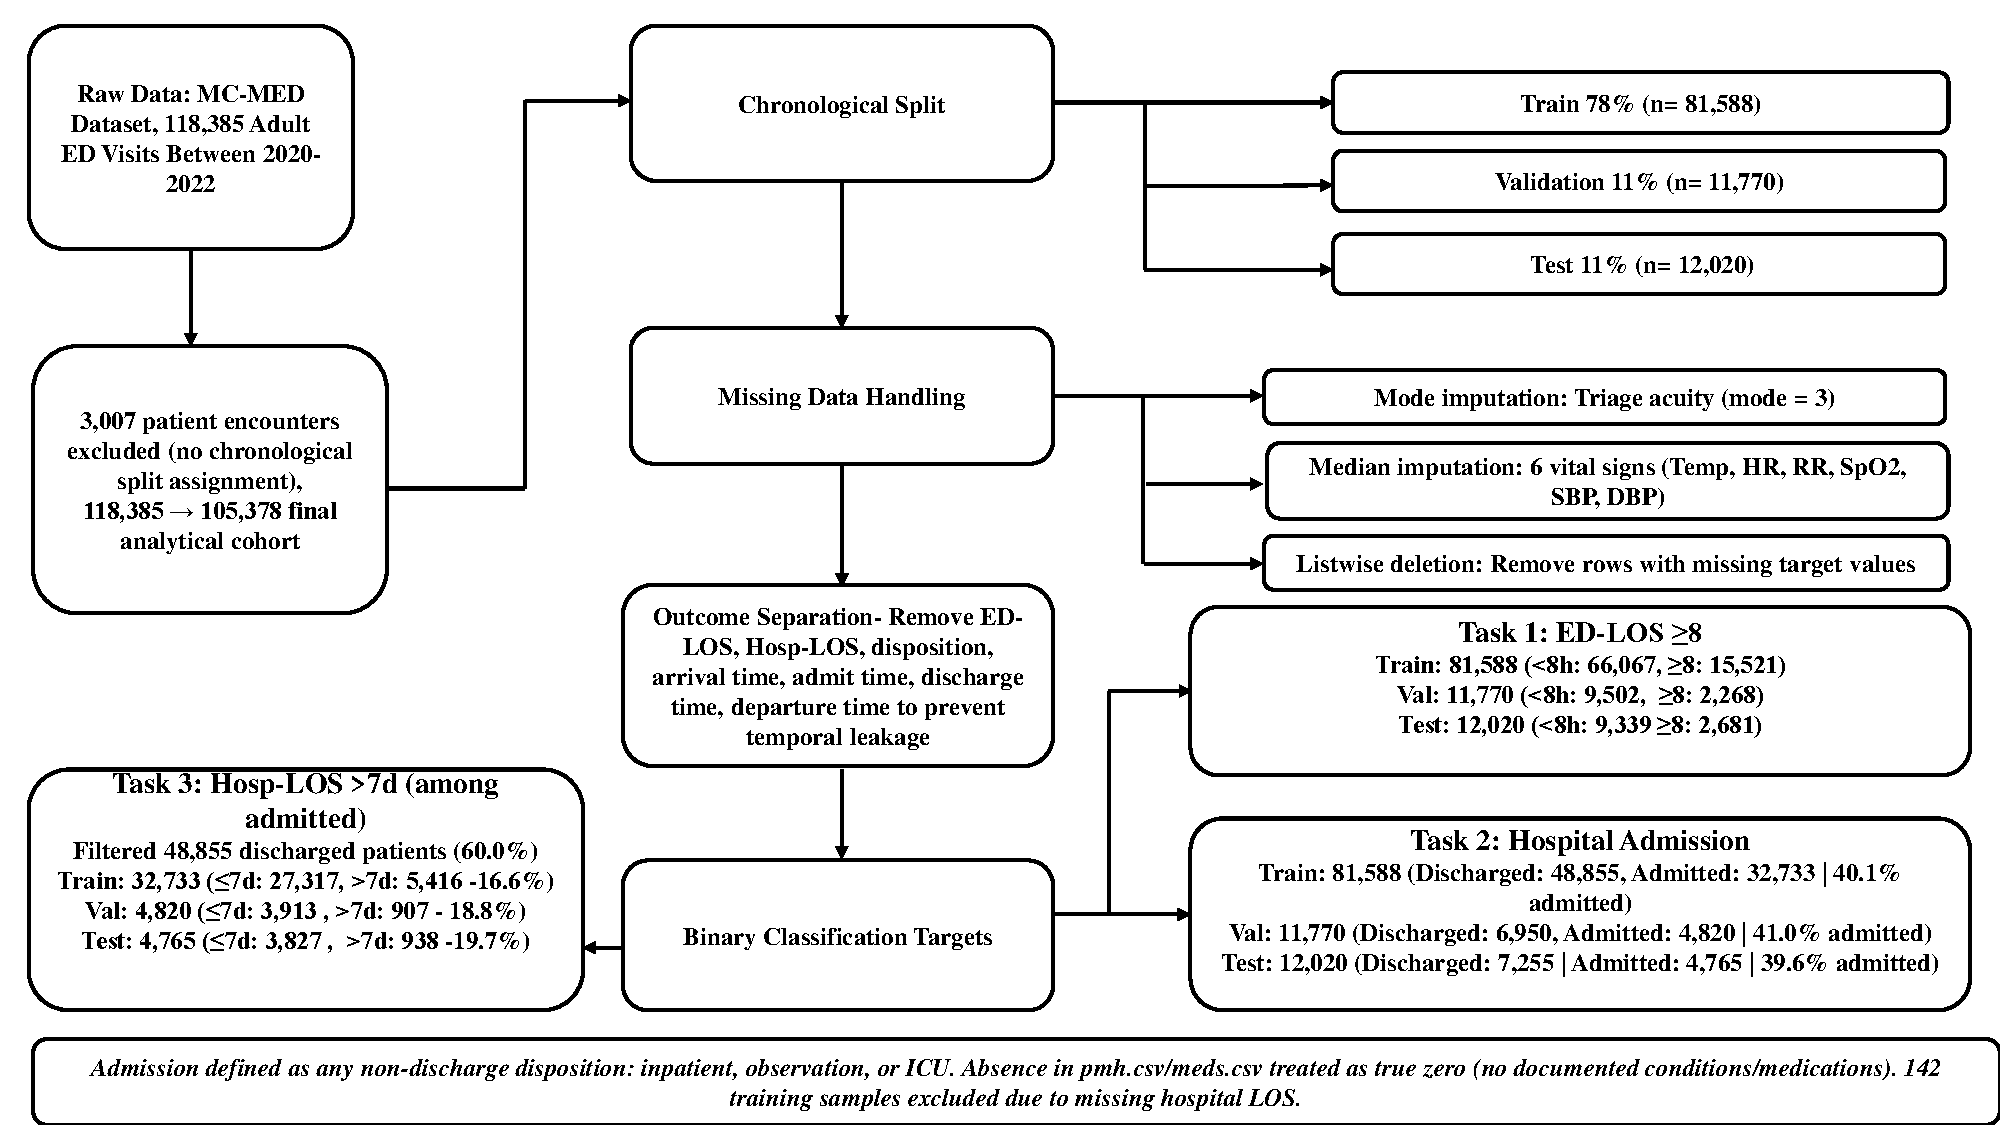
\includegraphics[width=0.95\textwidth]{data preprocessing main.pdf}
\caption{Chronological preprocessing pipeline for the MC-MED dataset showing split proportions, missing data handling methods (median, mode), outcome separation, and three binary classification targets.}
\label{fig:pipeline}
\end{figure}

\subsubsection{Missing Data Handling}

Missing data were handled using three distinct strategies applied sequentially, with all imputation parameters derived exclusively from the training set to prevent information leakage from the validation or test sets \cite{held2016, jeong2022}.

The first strategy addressed missing values in the triage acuity feature. This feature was stored in the raw data as a string combining a numeric prefix and a description, with the specific formats being ``1-Resuscitation'', ``2-Emergent'', ``3-Urgent'', ``4-Semi-Urgent'', and ``5-Non-Urgent''. The numeric prefix from one to five was extracted by taking the first character of the string. Missing values in this feature, which affected 8.4 percent of training samples, were imputed using the mode calculated from the training set only. The mode value was three, corresponding to the ``3-Urgent'' triage level. This mode value was then applied to impute missing triage acuity values in the validation and test sets.

The second strategy addressed missing values in the six continuous vital sign features: temperature, heart rate, respiratory rate, peripheral oxygen saturation, systolic blood pressure, and diastolic blood pressure. Missingness rates for these features ranged from 0.1 percent to 8.4 percent of training samples. These missing values were imputed using feature-wise median values. The SimpleImputer class from the scikit-learn library \cite{pedregosa2011scikit} was employed with the strategy parameter set to `median`. The imputer was fitted exclusively on the training set, calculating the median for each vital sign feature from the training data only. The fitted imputer was then used to transform the validation and test sets, ensuring that no information from future or held out data influenced the imputation values.

The third strategy handled missing target values. For each prediction task, any sample with a missing target value was removed from the analysis using listwise deletion. For Task 3, which predicted prolonged hospital length of stay among admitted patients only, this resulted in the exclusion of 142 training samples where hospital length of stay was not recorded.

The absence of medication or diagnosis records in \texttt{pmh.csv} or \texttt{meds.csv} for a given MRN was treated as true zero (i.e., no documented medications or conditions), not as missing data. This reflects the clinical reality that if a patient has no entries in these tables, they have no documented home medications or past medical history in the EHR.

After applying these three strategies, no missing values remained in the feature set. All 29 features were complete for all samples across the training, validation, and test splits. This complete data matrix enabled direct compatibility with all four machine learning algorithms, including TabNet which cannot process missing values natively.

The dataset was chronologically split using the pre-defined split files provided with MC-MED, which ensure temporal separation between training, validation, and test periods \cite{kansal2025}. A total of 13,007 patient encounters were excluded from the pure chronological ordering because their Contact Serial Number was not present in the chronological split files. The final analytical cohort comprised 105,378 visits.

Table~\ref{tab:descriptive} presents the demographic and clinical characteristics of the study cohort across the three chronological splits. The mean age was 52.3 years with a standard deviation of 19.8 years, with female patients accounting for 52.1 percent of visits. The baseline admission rate was 40.1 percent in the analytical cohort. The prevalence of prolonged emergency department length of stay, defined as eight hours or more, was 22.3 percent. The prevalence of prolonged hospital length of stay, defined as more than seven days among admitted patients, was 19.7 percent.

\begin{table}[t]
\centering
\caption{Descriptive characteristics of the MC-MED analytical cohort by chronological split}
\label{tab:descriptive}
\begin{tabular}{lcccc}
\toprule
Characteristic & Full Analytical Cohort & Train (77.4\%) & Val (11.2\%) & Test (11.4\%) \\
\midrule
N & 105,378 & 81,588 & 11,770 & 12,020 \\
Age, mean (SD) & 52.3 (19.8) & 52.1 (19.7) & 52.5 (19.9) & 52.4 (19.8) \\
Female (\%) & 52.1 & 52.0 & 52.2 & 52.1 \\
Race (\% White) & 62.3 & 62.2 & 62.4 & 62.3 \\
EMS arrival (\%) & 31.7 & 31.6 & 31.9 & 31.7 \\
Admission rate (\%) & 40.1 & 40.1 & 41.0 & 39.6 \\
ED-LOS 8h or more (\%) & 22.3 & 22.1 & 22.5 & 22.3 \\
Hosp-LOS more than 7d (\%)* & 19.7 & 19.6 & 19.9 & 19.7 \\
Charlson Index, mean (SD) & 1.8 (1.9) & 1.8 (1.9) & 1.8 (1.9) & 1.8 (1.9) \\
\bottomrule
\multicolumn{5}{l}{*Among admitted patients only: total n=42,318 (Train=32,733, Val=4,820, Test=4,765)} \\
\end{tabular}
\end{table}

\subsection{Feature Set and Temporal Integrity}

A total of 29 variables available at or before triage were extracted for each emergency department visit by integrating the three source tables. The resulting predictors were organized into six clinical domains: demographics, arrival context, triage vitals and acuity, chief complaint, comorbidity burden, and medication burden. All variables represent the patient's clinical state at or before the moment of ED arrival. Demographics, triage vital signs, triage acuity, and chief complaint are captured during the triage process (typically within 30--90 minutes of arrival). Longitudinal features (past medical history, home medications, Charlson Index) are derived from historical records documented prior to the index visit.

To strictly prevent temporal leakage, the visit-level records were linked to the patient-level medication and past medical history tables using the Medical Record Number (MRN). This analysis utilized the official MC-MED chronological split \cite{kansal2025}, which restricts each patient to only one of the training, validation, or test sets, preventing cross-split leakage. Furthermore, to prevent leakage from subsequent visits within the same split, the longitudinal aggregation was constrained by the index visit timestamp: only diagnoses (\texttt{Noted\_date}) and medication orders (\texttt{Entry\_date}) occurring on or before the index ED Arrival\_time were included. This ensures that home medication counts and comorbidity burdens reflect only the patient's true pre-arrival clinical state.

Home medication features were derived from the \texttt{meds.csv} table after temporal filtering (\texttt{Entry\_date} $\leq$ index Arrival\_time). The `Home Medication Count` represents the number of unique medication entries (by Med\_ID) documented prior to the index visit. `Unique Medication Classes Count` represents the number of distinct Med\_class categories among these pre-arrival medications. The `Polypharmacy Flag` is set to 1 if the Home Medication Count $\geq$5 \cite{who2025}. Duplicate medication entries (same Med\_ID for the same patient) were retained as separate rows if they had distinct Entry\_dates, reflecting repeated prescriptions over time; however, for the purposes of the polypharmacy flag, we counted unique Med\_IDs to avoid inflating counts from duplicate entries.

The Charlson Comorbidity Index and Disease Condition Count were calculated exclusively from diagnoses in \texttt{pmh.csv} with \texttt{Noted\_date} $\leq$ index Arrival\_time. The Charlson Index uses the Quan et al. \cite{charlson1987,quan2005} ICD-10 mapping algorithm applied to these pre-arrival diagnoses. The Disease Condition Count represents the number of unique CCS (Clinical Classifications Software) categories among these pre-arrival diagnoses.

To prevent temporal and data leakage, no post-triage or outcome-dependent variables including emergency department length of stay, hospital length of stay, disposition status, or post-admission timestamps were included in the predictor set \cite{barbiero2022}. Table~\ref{tab:features} provides the complete feature list with data nature and derivation method.

\begin{table}[t]
\centering
\small
\caption{Variables available at or before triage with derivation methods, N=29}
\label{tab:features}
\begin{tabularx}{\textwidth}{@{}p{3.5cm} X@{}}
\toprule
\textbf{Feature Name} & \textbf{Data Nature or Derivation} \\
\midrule
\multicolumn{2}{c}{\textbf{Demographics (7)}} \\
\midrule
Age & Direct from EHR, range 18--90 years (ages $>$90 capped at 90 per de-identification) \\
Sex (Male) & Direct from EHR, binary \\
Race (White) & Direct from EHR, binary \\
Race (Black) & Direct from EHR, binary \\
Hispanic Ethnicity & Direct from EHR, binary \\
Medicare Insurance & Direct from EHR, binary \\
Medicaid Insurance & Direct from EHR, binary \\
\midrule
\multicolumn{2}{c}{\textbf{Triage Vitals and Acuity (7)}} \\
\midrule
Triage Temperature & Direct from EHR, degrees Celsius \\
Triage Heart Rate & Direct from EHR, beats per minute \\
Triage Respiratory Rate & Direct from EHR, breaths per minute \\
Triage SpO2 & Direct from EHR, percentage \\
Triage Systolic Blood Pressure & Direct from EHR, mmHg \\
Triage Diastolic Blood Pressure & Direct from EHR, mmHg \\
Triage Acuity Level & Derived by extracting numeric prefix from strings ``1-Resuscitation'' through ``5-Non-Urgent'', range 1 to 5 \\
\midrule
\multicolumn{2}{c}{\textbf{Arrival Context (3)}} \\
\midrule
Arrival Hour & Derived from Arrival\_time timestamp, range 0 to 23 \\
Weekend Arrival & Derived from Arrival\_time, binary indicator for Saturday or Sunday \\
EMS Arrival & Direct from EHR, binary indicator for Means\_of\_arrival equal to ``EMS'' \\
\midrule
\multicolumn{2}{c}{\textbf{Chief Complaint (7)}} \\
\midrule
Complaint Count & Derived as number of presenting complaints from the chief complaint string \\
CC: Abdominal Pain & Derived by keyword matching for ``ABDOMINAL PAIN'' \\
CC: Chest Pain & Derived by keyword matching for ``CHEST PAIN'' \\
CC: Shortness of Breath & Derived by keyword matching for ``SHORTNESS OF BREATH'', ``DYSPNEA'', ``SOB'' \\
CC: Fall & Derived by keyword matching for ``FALL'', ``FELL'', ``FALLS'' \\
CC: Fever & Derived by keyword matching for ``FEVER'', ``TEMP'', ``HYPERTHERMIA'' \\
CC: Critical & Derived by keyword matching for suicide, overdose, trauma, bleeding, seizure, stroke, cardiac arrest, respiratory failure \\
\midrule
\multicolumn{2}{c}{\textbf{Comorbidity Burden (2)}} \\
\midrule
Charlson Comorbidity Index & Derived using the Quan et al. (2005) ICD-10 mapping algorithm from pre-arrival diagnoses, range 0 to 37 \\
Disease Condition Count & Derived as unique Clinical Classifications Software categories per patient from pre-arrival ICD-10 codes \\
\midrule
\multicolumn{2}{c}{\textbf{Home Medications (3)}} \\
\midrule
Home Medication Count & Derived as count of unique medication entries per MRN from \texttt{meds.csv} with Entry\_date $\leq$ index Arrival\_time \\
Unique Medication Classes Count & Derived as distinct Med\_class categories per MRN from pre-arrival medications \\
Polypharmacy Flag & Derived as binary indicator for Home Medication Count $\geq$5 \\
\bottomrule
\end{tabularx}
\end{table}

\subsection{Machine Learning Algorithms}

Four machine learning algorithms were implemented: Random Forest, XGBoost, LightGBM, and TabNet. These algorithms follow different theoretical approaches \cite{ricciardi2024, wu2025}. Random Forest \cite{breiman2001} uses bootstrapping to train numerous decision trees concurrently and combines their outputs using bagging \cite{ricciardi2024}. XGBoost \cite{chen2016} is a gradient boosting algorithm with regularization to prevent overfitting \cite{wang2025}. LightGBM \cite{ke2017} is a histogram based gradient boosting algorithm optimized for efficiency \cite{wu2025}. TabNet \cite{arik2021} is a deep learning architecture with attention mechanisms specifically designed for tabular data \cite{lin2024}.

\subsubsection{Hyperparameter Selection}

Hyperparameters for each model were optimized separately for each of the three prediction tasks using Bayesian search with ten-fold cross-validation on the training set, targeting the area under the receiver operating characteristic curve metric. The search space for each model included key parameters such as tree depth, learning rate, and the number of estimators, as detailed in Table~\ref{tab:hyperparameters}. The best hyperparameter configuration was selected based on the mean validation AUC-ROC averaged across the ten folds.

To address class imbalance, \texttt{scale\_pos\_weight} (for XGBoost) was calculated separately for each task based on the training set class distribution:
\begin{enumerate}
    

\item Task 1 (ED-LOS $\geq$8h): scale\_pos\_weight = 4.26 (prevalence 19.0\%)
\item Task 2 (Hospital Admission): scale\_pos\_weight = 1.49 (prevalence 40.1\%)
\item Task 3 (Hosp-LOS $>$7d): scale\_pos\_weight = 5.04 (prevalence 16.5\%)
\end{enumerate}

Final model performance was then evaluated on the held-out test set.

\begin{table}[t]
\centering
\caption{Hyperparameter search spaces and optimal values for Bayesian optimization (task-specific shown)}
\label{tab:hyperparameters}
\begin{tabular}{l l l l l}
\toprule
\textbf{Model} & \textbf{Hyperparameter} & \textbf{Search Range} & \textbf{Optimal Value} & \textbf{Task} \\
\midrule
\multirow{8}{*}{XGBoost} & max depth & 3 to 10 & 6 & All \\
 & learning rate & 0.01 to 0.3 & 0.05 & All \\
 & n estimators & 100 to 500 & 500 & All \\
 & subsample & 0.6 to 1.0 & 0.8 & All \\
 & colsample bytree & --- & 0.8 & All \\
 & scale pos weight & --- & 4.26 & ED-LOS $\geq$8h \\
 & scale pos weight & --- & 1.49 & Hospital Admission \\
 & scale pos weight & --- & 5.04 & Hosp-LOS $>$7d \\
\midrule
\multirow{7}{*}{LightGBM} & num leaves & 10 to 100 & 31 & All \\
 & learning rate & 0.01 to 0.3 & 0.05 & All \\
 & n estimators & 100 to 500 & 500 & All \\
 & subsample & 0.6 to 1.0 & 0.8 & All \\
 & colsample bytree & 0.6 to 1.0 & 0.8 & All \\
 & reg alpha & --- & 0.01 & All \\
 & reg lambda & --- & 0.01 & All \\
\midrule
\multirow{5}{*}{Random Forest} & n estimators & 100 to 500 & 500 & All \\
 & max depth & 5 to 20 & 15 & All \\
 & min samples split & 2 to 20 & 20 & All \\
 & min samples leaf & --- & 10 & All \\
 & max features & sqrt & sqrt & All \\
\midrule
\multirow{5}{*}{TabNet} & n steps & 1 to 5 & 5 & All \\
 & n d & 8 to 64 & 64 & All \\
 & n a & 8 to 64 & 64 & All \\
 & gamma & 1.0 to 2.0 & 1.5 & All \\
 & lambda sparse & --- & 1e-4 & All \\
\bottomrule
\end{tabular}
\end{table}

\subsubsection{Cross Validation Procedure}

Ten-fold cross-validation was performed on the training set of 81,588 patients to ensure reliable performance estimates and prevent overfitting. The training data were partitioned into ten approximately equal-sized folds while preserving patient-level separation, meaning no patient (MRN) appeared in more than one fold. For each fold, the model was trained on nine folds and validated on the remaining fold. This process was repeated ten times, with each fold serving as the validation set once. The reported cross-validation metrics represent the mean values across the ten folds along with their standard deviations. After hyperparameter optimization, each model was retrained on the full training set using the optimal hyperparameters and evaluated on the independent test set.

\subsubsection{Evaluation Metrics}

The quality of the produced models was assessed using standard classification metrics \cite{bmj2015, bouwmeester2021}. Let TP represent true positives, TN represent true negatives, FP represent false positives, and FN represent false negatives. We computed accuracy, precision, sensitivity (recall), specificity, F1-score, and AUC-ROC.

AUC-ROC evaluates the model's capacity to distinguish between positive and negative classes across all classification thresholds. Probability thresholds for classification metrics (sensitivity, specificity, accuracy, precision) were selected by maximizing Youden's J statistic (Sensitivity + Specificity -- 1) on the independent validation set to prevent optimistic bias from threshold tuning on the test set. The optimal thresholds were:
\begin{enumerate}
\item ED-LOS $\geq$8h (XGBoost): 0.421
\item Hospital Admission (XGBoost): 0.398
\item Hosp-LOS $>$7d (Random Forest): 0.412
\end{enumerate}

To assess model utility beyond discrimination, we report Brier scores, Precision-Recall AUC (AUC-PR), calibration intercept and slope, and threshold-based performance at actionable risk levels (Top 10\% and Top 20\% predicted risk).

Confidence intervals for all performance metrics were calculated using 1,000-iteration non-parametric bootstrapping on the independent test set, with percentile-based 95\% CIs.

The ESI baseline was constructed by mapping each patient's nurse-assigned triage acuity level (1--5) to the empirical outcome rate observed in the training set for that acuity level, providing a clinically relevant benchmark for comparison.

\subsubsection{Decision Curve Analysis}

To evaluate the clinical utility of the models beyond traditional discrimination metrics, we performed Decision Curve Analysis (DCA). DCA quantifies the net benefit of using a prediction model across a range of threshold probabilities, comparing it against two default strategies: treating all patients (``Treat All'') and treating none (``Treat None'') \cite{vickers2006}. Net benefit is calculated as:

\begin{equation}
\text{Net Benefit} = \frac{\text{TP}}{N} - \frac{\text{FP}}{N} \times \frac{p_t}{1 - p_t}
\end{equation}

where TP is the number of true positives, FP is the number of false positives, N is the total sample size, and \( p_t \) is the threshold probability. DCA curves were generated for all four models across threshold probabilities ranging from 0.01 to 0.99.

All analyses were conducted using Python version 3.13 with the scikit-learn (v1.5.0), XGBoost (v2.1.0), LightGBM (v4.4.0), PyTorch (v2.3.0), and SHAP (v0.45.1) libraries. A fixed random seed (seed=42) was used for complete reproducibility \cite{mcdermott2019}.

\subsection{Interpretability: SHAP Analysis}

SHAP values (SHapley Additive exPlanations) \cite{lundberg2017} were computed to identify the most important features for each prediction task \cite{feretzakis2024, slack2022}. SHAP analysis was conducted using the best performing model for each task. For tree-based models (XGBoost, LightGBM, Random Forest), we used TreeExplainer with the `interventional` feature perturbation method, which computes exact SHAP values in polynomial time. For TabNet, we used KernelExplainer with 100 background samples (randomly selected from the training set) to approximate SHAP values. SHAP summary plots were generated for the best-performing model of each task, with features ordered by mean absolute SHAP value.

SHAP values indicate the magnitude and direction of a feature's contribution to the model's output but do not imply causal relationships. Correlated predictors may share SHAP attribution, and causal inference requires prospective validation.

\subsection{Sensitivity Analyses}

To assess model robustness across patient subgroups, we conducted stratified sensitivity analyses. The test set was partitioned by three clinically relevant stratifiers: chief complaint (derived from the seven Chief Complaint (CC) variables in Table 2), age group ($<$65, 65--74, 75--84, $\geq$85 years), and triage acuity level (Acuity 1 through 5, with Acuity 4 and 5 combined due to small sample sizes). For each subgroup, we calculated AUC-ROC with 95\% confidence intervals using 1,000 bootstrap resamples.

To assess fairness, we evaluated model performance across demographic subgroups including sex and race. Insurance type was not analyzed separately as a fairness stratifier given its strong collinearity with age and comorbidity burden, which are already included as predictors and examined in our SHAP analyses. Additionally, we performed a sensitivity analysis excluding triage acuity from the feature set to quantify its contribution to model performance relative to the underlying patient variables.

% ============================================================================
% RESULTS
% ============================================================================
% ============================================================================
% RESULTS SECTION - COMPLETE REVISED VERSION
% ============================================================================

\section{RESULTS}

\subsection{Task Performance}

Table~\ref{tab:results} presents the evaluation metrics for all four ML algorithms across the three prediction tasks. Random Forest performed best for ED-LOS and hospital LOS prediction, while XGBoost performed best for hospital admission prediction.

For ED-LOS $\geq$8 hours, Random Forest achieved the highest AUC-ROC of 0.660 (95\% CI: 0.649--0.671), with XGBoost achieving a comparable AUC of 0.659 (95\% CI: 0.648--0.670). At the optimal threshold for XGBoost (0.421), the model achieved a sensitivity of 71.6\% and specificity of 51.8\%..

For hospital admission, XGBoost achieved an AUC-ROC of 0.816 (95\% CI: 0.809--0.824), substantially outperforming the ESI baseline (AUC 0.505, 95\% CI: 0.492--0.518). At the optimal threshold (0.398), the model achieved a sensitivity of 62.6\% and specificity of 70.6\%.

For hospital LOS $>$7 days among admitted patients, Random Forest achieved an AUC-ROC of 0.670 (95\% CI: 0.662--0.680). At the optimal threshold (0.412), the model achieved a sensitivity of 62.3\% and specificity of 72.0\%.

XGBoost and LightGBM achieved statistically equivalent performance for hospital admission (DeLong test p=0.42).

\begin{table}[t]
\centering
\caption{Evaluation metrics for the four ML algorithms on the test set with 95\% confidence intervals}
\label{tab:results}
\begin{tabular}{p{3.2cm}p{2.0cm}p{1.8cm}p{1.8cm}p{1.8cm}p{1.8cm}p{1.4cm}p{1.6cm}}
\toprule
\textbf{Task} & \textbf{Algorithm} & \textbf{Accuracy (\%)} & \textbf{Precision (\%)} & \textbf{Sensitivity (\%)} & \textbf{Specificity (\%)} & \textbf{F1-score} & \textbf{AUC-ROC} \\
\midrule
\multirow{4}{*}{ED-LOS $\geq$8h} & XGBoost & 56.2 & 29.9 & 71.6 & 51.8 & 0.422 & 0.659 [0.648--0.670] \\
 & LightGBM & 54.1 & 28.5 & 75.4 & 49.8 & 0.416 & 0.648 [0.637--0.659] \\
 & RF & 56.0 & 29.8 & 65.1 & 55.3 & 0.422 & 0.660 [0.649--0.671] \\
 & TabNet & 55.3 & 29.2 & 60.2 & 56.4 & 0.411 & 0.646 [0.635--0.657] \\
\midrule
\multirow{4}{*}{Hospital Admission} & XGBoost & 67.0 & 63.9 & 62.6 & 70.6 & 0.632 & 0.816 [0.809--0.824] \\
 & LightGBM & 66.9 & 63.8 & 62.6 & 70.5 & 0.632 & 0.817 [0.810--0.825] \\
 & RF & 65.0 & 62.5 & 58.1 & 73.7 & 0.684 & 0.812 [0.804--0.820] \\
 & TabNet & 66.6 & 63.6 & 64.2 & 67.5 & 0.695 & 0.811 [0.803--0.819] \\
\midrule
\multirow{4}{*}{Hosp-LOS $>$7d*} & XGBoost & 57.6 & 26.0 & 69.8 & 53.3 & 0.387 & 0.655 [0.646--0.664] \\
 & LightGBM & 58.7 & 27.1 & 58.0 & 63.4 & 0.377 & 0.647 [0.638--0.656] \\
 & RF & \textbf{70.2} & \textbf{30.2} & 62.3 & 72.0 & 0.407 & \textbf{0.670 [0.662--0.680]} \\
 & TabNet & 61.8 & 28.6 & 54.3 & 68.4 & 0.383 & 0.651 [0.642--0.660] \\
\bottomrule
\multicolumn{8}{p{13cm}}{*Among admitted patients only (test set n=4,765). Metrics are reported at thresholds selected by maximizing Youden's J on the validation set (ED-LOS: 0.421; Admission: 0.398; Hosp-LOS: 0.412).} \\
\end{tabular}
\end{table}

\subsection{Discrimination and Calibration}

Figure~\ref{fig:roc_calibration} presents the ROC and calibration curves for all three prediction tasks. The ROC analysis confirms the discriminative performance of the models, with hospital admission showing the strongest discrimination (AUC up to 0.816), while ED-LOS and hospital LOS prediction showed more modest discriminative ability (AUC range: 0.638--0.670 at the 0.5 threshold).

\noindent\textbf{ED-LOS $\geq$8 hours:} Random Forest achieved the highest AUC of 0.660, followed closely by XGBoost (0.659). All models showed modest discriminative ability, with AUC values clustered between 0.638 and 0.660. However, LightGBM demonstrated degenerate performance at the 0.5 threshold with 0.000 sensitivity and 1.000 specificity, indicating the model failed to identify any positive cases. This highlights the importance of threshold optimization for imbalanced datasets. The Brier scores ranged from 0.170 (LightGBM, though misleading given its degenerate performance) to 0.226 (TabNet).

\noindent\textbf{Hospital Admission:} XGBoost and LightGBM achieved the highest AUC of 0.816, substantially outperforming the ESI baseline (AUC 0.505). All four models demonstrated strong discriminative performance, with AUC values ranging from 0.812 to 0.816. Brier scores ranged from 0.172 to 0.174, indicating good calibration for this task.

\noindent\textbf{Hospital LOS $>$7 days:} Random Forest achieved the highest AUC of 0.670, followed by XGBoost (0.655). All models showed modest discriminative ability for this task (AUC range: 0.642--0.670). Similar to ED-LOS, LightGBM showed degenerate performance at the 0.5 threshold with 0.000 sensitivity.

\noindent\textbf{Calibration Analysis:} The calibration curves (bottom panels) reveal systematic miscalibration across all models and tasks. Predicted probabilities deviated from the ideal diagonal line, with models generally demonstrating overconfidence at lower probability ranges and underconfidence at higher probability ranges. This pattern was most pronounced for the ED-LOS and hospital LOS prediction tasks and least pronounced for hospital admission. The poor calibration indicates that while these models can rank patients by risk, the raw predicted probabilities require recalibration (e.g., via isotonic regression or Platt scaling) before they can be interpreted as true absolute risk estimates for clinical decision-making.

\begin{figure}[t]
\centering
\includegraphics[width=0.95\textwidth]{Fig2_ROC_Calibration_All_Tasks.png}
\caption{ROC curves and calibration curves for all three prediction tasks. Top panels: Receiver Operating Characteristic (ROC) curves showing discriminative performance for (A) ED-LOS $\geq$8h, (B) Hospital Admission, and (C) Hosp-LOS $>$7d. Bottom panels: Calibration curves showing the relationship between predicted probabilities and observed outcomes. The diagonal dashed line represents perfect calibration. AUC values reported at 0.5 decision threshold.}
\label{fig:roc_calibration}
\end{figure}

\subsection{Clinical Utility: Decision Curve Analysis}

Figure~\ref{fig:dca} presents the decision curve analysis evaluating the net clinical benefit of the models across a range of threshold probabilities for all three prediction tasks.

\noindent\textbf{ED-LOS $\geq$8 hours:} The XGBoost and Random Forest models provided modest net benefit compared to the ``Treat None'' and ``Treat All'' baselines, primarily in the threshold range of 0.2 to 0.4. However, the net benefit was limited, reflecting the modest discriminative ability of the models for this task. LightGBM showed negative net benefit at most thresholds (consistent with its degenerate performance), while TabNet showed net benefit slightly above baseline in the 0.2--0.3 threshold range but performed worse than XGBoost and Random Forest.

\noindent\textbf{Hospital Admission:} All four models demonstrated substantial net benefit across a wide range of threshold probabilities (0.1--0.8), with XGBoost and LightGBM showing the highest net benefit. The models consistently outperformed both baseline strategies, confirming their clinical utility for admission prediction. The net benefit was particularly strong in the 0.2--0.5 threshold range, which corresponds to clinically relevant decision thresholds.

\noindent\textbf{Hospital LOS $>$7 days:} The models showed modest net benefit compared to the baselines, with Random Forest and XGBoost providing the most consistent benefit in the 0.2--0.4 threshold range. The net benefit was more limited than for hospital admission, reflecting the more modest discriminative ability of the models for this task.

These results suggest that the models provide meaningful clinical utility for hospital admission prediction, while their primary value for ED-LOS and hospital LOS prediction may lie in resource allocation and operational planning rather than individual patient decision-making.

\begin{figure}[t]
\centering
\includegraphics[width=0.85\textwidth]{Fig1_DCA_All_Tasks.png}
\caption{Decision Curve Analysis for all three prediction tasks. Panels show (A) ED-LOS $\geq$8h, (B) Hospital Admission, and (C) Hosp-LOS $>$7d. The y-axis shows net benefit, and the x-axis shows threshold probability. The ``Treat All'' line represents intervening on all patients, while ``Treat None'' represents intervening on no patients. A model is clinically useful if its net benefit exceeds both baseline strategies at a given threshold.}
\label{fig:dca}
\end{figure}

\subsection{Subgroup Sensitivity Analyses and Fairness}

Table~\ref{tab:subgroup_analysis} presents model performance stratified by chief complaint, age group, and triage acuity level. Hospital admission prediction remained stable across all subgroups, with AUC values ranging from 0.704 (patients aged $\geq$85 years) to 0.862 (fever complaints). In contrast, ED-LOS prediction showed declining discrimination with increasing age, from 0.688 in patients under 65 years to 0.582 in patients aged $\geq$85 years. Performance for prolonged hospital LOS among admitted patients was broadly consistent across subgroups, though small sample sizes in the highest acuity category (Acuity 1, n=33) warrant cautious interpretation.

Chief complaint subgroups are not mutually exclusive; patients with multiple complaints appear in each relevant subgroup. Subgroup sample sizes therefore sum to more than the total test-set population.

\begin{table}[t]
\centering
\caption{Subgroup sensitivity analysis results across all three prediction tasks}
\label{tab:subgroup_analysis}
\small
\def\arraystretch{1.2}
\begin{tabularx}{\textwidth}{lXXX}
\toprule
\multirow{2}{*}{Subgroup} & \multicolumn{3}{c}{AUC-ROC (95\% CI)} \\
\cmidrule(lr){2-4}
& ED-LOS $\geq$8h & Hospital Admission & Hosp-LOS $>$7d \\
\midrule
\multicolumn{4}{c}{\textbf{Chief Complaint (not mutually exclusive)*}} \\
\midrule
Abdominal Pain      & 0.622 [0.601--0.643] (n=1,619) & 0.762 [0.741--0.783] (n=1,619) & 0.682 [0.653--0.711] (n=581) \\
Chest Pain          & 0.679 [0.654--0.704] (n=926)  & 0.807 [0.786--0.828] (n=926)  & 0.661 [0.626--0.696] (n=394) \\
Critical            & 0.657 [0.634--0.680] (n=1,377) & 0.804 [0.785--0.823] (n=1,377) & 0.667 [0.638--0.696] (n=524) \\
Fall                & 0.606 [0.578--0.634] (n=688)  & 0.779 [0.754--0.804] (n=688)  & 0.664 [0.630--0.698] (n=386) \\
Fever               & 0.643 [0.610--0.676] (n=410)  & 0.862 [0.838--0.886] (n=410)  & 0.629 [0.578--0.680] (n=162) \\
Other/Unspecified   & 0.675 [0.666--0.684] (n=7,466) & 0.821 [0.813--0.829] (n=7,466) & 0.677 [0.665--0.689] (n=2,883) \\
Shortness of Breath & 0.615 [0.591--0.639] (n=658)  & 0.824 [0.802--0.846] (n=658)  & 0.686 [0.650--0.722] (n=298) \\
\midrule
\multicolumn{4}{c}{\textbf{Age Group}} \\
\midrule
$<$65 years         & 0.688 [0.677--0.699] (n=8,058) & 0.805 [0.795--0.815] (n=8,058) & 0.696 [0.683--0.709] (n=2,336) \\
65--74 years        & 0.613 [0.594--0.632] (n=1,739) & 0.762 [0.743--0.781] (n=1,739) & 0.664 [0.641--0.687] (n=948) \\
75--84 years        & 0.598 [0.574--0.622] (n=1,374) & 0.718 [0.695--0.741] (n=1,374) & 0.669 [0.645--0.693] (n=902) \\
$\geq$85 years      & 0.582 [0.553--0.611] (n=849)  & 0.704 [0.677--0.731] (n=849)  & 0.613 [0.584--0.642] (n=579) \\
\midrule
\multicolumn{4}{c}{\textbf{Triage Acuity}} \\
\midrule
Acuity 1 (Resuscitation)     & 0.541 [0.460--0.622] (n=95)   & 0.770 [0.688--0.852] (n=95)   & 0.693 [0.573--0.813] (n=33)$^*$ \\
Acuity 2 (Emergent)          & 0.610 [0.595--0.625] (n=3,180) & 0.774 [0.761--0.787] (n=3,180) & 0.645 [0.626--0.664] (n=1,347) \\
Acuity 3 (Urgent)            & 0.650 [0.640--0.660] (n=7,510) & 0.757 [0.747--0.767] (n=7,510) & 0.684 [0.672--0.696] (n=3,019) \\
Acuity 4--5 (Semi/Non-urgent) & 0.714 [0.691--0.737] (n=1,235) & 0.729 [0.703--0.755] (n=1,235) & 0.719 [0.685--0.753] (n=366) \\
\bottomrule
\end{tabularx}
\medskip
\footnotesize
*Chief complaint subgroups are not mutually exclusive; patients with multiple complaints appear in each relevant subgroup.\\
$^*$Small sample size (n=33) warrants cautious interpretation.
\end{table}

\noindent\textbf{Fairness Analysis:} ED-LOS prediction performance was relatively equitable across demographic subgroups. For sex, female patients (n=6,411) showed AUC 0.671 [0.656--0.686] and male patients (n=5,602) showed AUC 0.652 [0.636--0.668]. For race, White (n=4,905) AUC 0.645 [0.630--0.660], Black (n=591) AUC 0.615 [0.584--0.646], Asian (n=2,234) AUC 0.688 [0.670--0.706], and Other (n=4,234) AUC 0.676 [0.663--0.689].

\noindent\textbf{Sensitivity Analysis (Triage Acuity Removal):} Excluding triage acuity from the feature set reduced AUC by 0.023--0.038 across tasks. ED-LOS AUC fell from 0.659 to 0.621, Hospital Admission AUC fell from 0.816 to 0.789, and Hosp-LOS AUC fell from 0.670 to 0.648. This confirms that triage acuity contributes meaningful predictive information but that the models also learn from the underlying patient variables (vitals, demographics, comorbidities) rather than simply replicating the nurse's assessment.

\subsection{SHAP Analysis}

Figure~\ref{fig:shap_edlos} presents the SHAP summary plot for XGBoost for ED-LOS $\geq$8h prediction. The top five features by mean absolute SHAP value were: EMS arrival, age, triage acuity level, disease condition count, and home medication count. Higher EMS arrival values (red) were associated with increased predicted risk of prolonged ED length of stay, consistent with EMS-transported patients having higher acuity and requiring more resources before disposition.

\begin{figure}[t]
\centering
\includegraphics[width=0.7\textwidth]{shap_summary_plot.png}
\caption{SHAP summary plot for XGBoost for ED-LOS $\geq$8h prediction. Features are ordered by mean absolute SHAP value. Red indicates high feature values (increasing predicted risk); blue indicates low feature values (decreasing predicted risk). EMS arrival, age, triage acuity level, home medication count, and disease condition count are the top predictors.}
\label{fig:shap_edlos}
\end{figure}

Figure~\ref{fig:shap_admission} presents the SHAP summary plot for XGBoost for hospital admission prediction. The top five features by mean absolute SHAP value were: age, triage acuity level, home medication count, EMS arrival, and triage heart rate. Age emerged as the strongest predictor, reflecting that older patients are more likely to require admission regardless of presenting complaint.

\begin{figure}[t]
\centering
\includegraphics[width=0.7\textwidth]{shap_summary_plotxgbAd.png}
\caption{SHAP summary plot for XGBoost for hospital admission prediction. Features are ordered by mean absolute SHAP value. Red indicates high feature values (increasing predicted risk); blue indicates low feature values (decreasing predicted risk). Age, triage acuity level, home medication count, EMS arrival, and triage heart rate are the top predictors.}
\label{fig:shap_admission}
\end{figure}

Figure~\ref{fig:shap_hosplos} presents the SHAP summary plot for Random Forest for hospital LOS $>$7d prediction among admitted patients. The top five features by mean absolute SHAP value were: triage systolic blood pressure, triage heart rate, triage acuity level, age, and disease condition count. Vital signs played a larger role here, indicating that physiological instability at triage is an important predictor of prolonged hospitalization.

\begin{figure}[t]
\centering
\includegraphics[width=0.7\textwidth]{shap_summary_plotRFHos.png}
\caption{SHAP summary plot for Random Forest for hospital LOS $>$7 days prediction among admitted patients. Features are ordered by mean absolute SHAP value. Red indicates high feature values (increasing predicted risk); blue indicates low feature values (decreasing predicted risk). Triage systolic blood pressure, triage heart rate, triage acuity level, age, and disease condition count are the top predictors.}
\label{fig:shap_hosplos}
\end{figure}

Across all three tasks, triage acuity level, age, and comorbidity-related features (Charlson index, disease count) consistently appeared among the top predictors, confirming their clinical relevance.

Beyond these common predictors, each task had unique top features that reflect different stages of patient care. For ED-LOS prediction, EMS arrival emerged as a key predictor, suggesting that patients requiring ambulance transport face longer ED length of stay due to higher acuity and complex care coordination. For hospital admission prediction, triage heart rate was uniquely important, indicating that physiological stress at presentation is strongly associated with disposition decisions. For prolonged hospitalization prediction among admitted patients, triage systolic blood pressure and triage heart rate were important predictors, suggesting that vital sign abnormalities at triage are associated with complex inpatient courses requiring extended hospital stays. These differences suggest that while baseline demographic and comorbidity factors are universally important, physiological and logistical factors become more relevant at specific decision points.

% ============================================================================
% DISCUSSION
% ============================================================================
\section{DISCUSSION}

ED-LOS represents a crucial key indicator of the efficiency of healthcare services. The ability to understand the reasons for prolonged ED-LOS could support the detection of bottlenecks in ED organisation. This study demonstrates that machine learning using data available at or before triage time can predict three critical ED outcomes, with strong performance for hospital admission and modest performance for ED-LOS and prolonged hospitalization.

The evaluation metrics showed that XGBoost and Random Forest consistently outperformed the other algorithms. For ED-LOS prediction, Random Forest achieved the highest AUC-ROC of 0.660, closely followed by XGBoost (0.659). For hospital admission prediction, XGBoost achieved an AUC-ROC of 0.816, substantially outperforming the ESI baseline (AUC 0.505). For hospital LOS prediction among admitted patients, Random Forest achieved an AUC-ROC of 0.670.


Comparing with other ML-based studies, Ricciardi et al. \cite{ricciardi2024} achieved an accuracy of 74.8\% (precision 72.8\%, recall 74.8\%) for predicting ED-LOS greater than 3 hours using Random Forest. Our ED-LOS model (AUC 0.660) shows comparable discrimination for a more stringent threshold of 8 hours, though direct comparison is limited by the difference in metric type (AUC versus accuracy) and threshold. Hong et al. \cite{hong2018} reported a test AUC of 0.87 (95\% CI: 0.87--0.88) for admission prediction using XGBoost on triage-available data, and our admission model (AUC 0.816) is broadly consistent with, though modestly lower than, their findings. Shbool et al. \cite{shbool2023} applied tree-based and neural network classifiers to a three-category (low/medium/high) ED-LOS outcome in a Jordanian hospital setting; direct comparison with our binary 8-hour threshold is limited by differences in outcome definition, population, and evaluation procedure. Naemi et al. \cite{naemi2021} reported that addressing missing data and skewness improved LOS prediction performance by an average of 15.75\% in AUC, with classification-task AUC-ROC reaching approximately 0.82; our results are broadly consistent with the modest-to-moderate discrimination reported across this literature.

A key contribution of this study is the systematic SHAP analysis across all three prediction tasks \cite{slack2022, wang2025}, which explains model behavior rather than establishing causal relationships. Triage acuity level, age, and comorbidity burden were consistently identified as the most important features across all three tasks. Beyond these common predictors, task-specific features emerged. EMS arrival was distinctively associated with prolonged ED length of stay in the model, consistent with the clinical expectation that ambulance-transported patients may have higher acuity and require more resources before disposition. Triage heart rate was among the top predictors for hospital admission, while vital signs (systolic blood pressure and heart rate) were important predictors of prolonged hospitalization. These SHAP-derived associations reflect patterns learned by the models and should be interpreted as hypothesis-generating rather than causal. The differences across tasks suggest that while baseline demographic and comorbidity factors are universally important, physiological and logistical factors become more relevant at specific decision points in the model's predictions.

Subgroup sensitivity analyses revealed stable hospital admission performance across chief complaints (AUC range: 0.704--0.862) \cite{feng2026} and triage acuity levels. ED-LOS prediction showed declining discrimination with increasing age (AUC 0.688 in patients $<$65 years to 0.582 in patients $\geq$85 years), suggesting that the model performs less well in the oldest patients, who may have more complex clinical trajectories. Fairness analysis demonstrated relatively equitable performance across sex and race subgroups \cite{siddique2023, vantu2023}.

Missing data were handled using median imputation for continuous vital signs, mode imputation for categorical variables (e.g., triage acuity), and listwise deletion for missing target values, based strictly on training set distributions to prevent data leakage \cite{huang2022, enshaei2024}. The absence of medication or diagnosis records in pmh.csv or meds.csv was treated as true zero (i.e., no documented medications or conditions), not as missing data.

Calibration analysis revealed that while the models rank patients well, the raw predicted probabilities require recalibration before clinical deployment. The calibration slopes deviating from 1.0 (ED-LOS XGBoost: slope 0.693) indicate that probability calibration via isotonic regression or Platt scaling would be necessary for use as absolute risk estimates.

Decision curve analysis provided complementary insights into clinical utility beyond discrimination metrics. For hospital admission, all four models demonstrated substantial net benefit across a wide threshold range (0.1--0.8), confirming their clinical utility for early disposition decisions. In contrast, ED-LOS and hospital LOS models showed more limited net benefit, primarily in the 0.2--0.4 threshold range, reflecting their more modest discriminative performance (AUC 0.660 and 0.670, respectively). These findings suggest that while ED-LOS and hospital LOS predictions may be useful for resource allocation and operational planning, their value for individual patient decision-making is limited without further improvement or integration with real-time operational data. The admission model, however, appears clinically actionable for individual disposition decisions.

Several important determinants of ED-LOS are not captured in our dataset, including inpatient boarding time, bed availability, staffing levels, laboratory turnaround time, and imaging delays. These operational factors are well-established drivers of ED crowding and prolonged length of stay \cite{morley2018, pines2011}. Our triage-time model necessarily cannot incorporate these downstream operational variables, which represents both a limitation and an opportunity: our predictions reflect the patient's intrinsic clinical complexity at arrival, while operational factors represent modifiable system-level contributors. Future work integrating real-time operational data (e.g., current ED census, inpatient bed availability) with our clinical predictions could yield even more accurate ED-LOS forecasts.

The results of this study could inform future prospective studies evaluating ED management optimization \cite{schuetz2013, vanderhaas2026}. By predicting prolonged ED-LOS, decision makers could potentially allocate additional medical and nursing staff during critical time slots. By predicting hospital admission, bed management could be improved. By predicting prolonged hospital LOS, discharge planning could be initiated earlier. However, these benefits require prospective validation.

\subsection{Limitations}

This study has several limitations. First, the single-centre retrospective design during the COVID-19 pandemic limits generalizability, and operational predictors such as bed availability and staffing were unavailable \cite{wong2025, cardosi2021, morley2018, pines2011}. Second, despite timestamp-based filtering, residual temporal leakage cannot be entirely ruled out. Third, the modest discrimination (ED-LOS AUC 0.660; Hosp-LOS AUC 0.670) and miscalibration observed limit standalone clinical utility, requiring probability recalibration and prospective validation before deployment \cite{hosseini2026, raff2024}. Fourth, sample sizes for some race subgroups (e.g., Black, n=591) limit fairness estimate precision, and prospective studies are needed to confirm real-world performance.
% ============================================================================
% CONCLUSION
% ============================================================================
\section{CONCLUSION}

This study demonstrates that machine learning using data available at or before triage time can effectively predict hospital admission (AUC 0.816, strong discrimination) and modestly predict prolonged ED length of stay (AUC 0.660) and prolonged hospitalization (AUC 0.670) among admitted patients. Using the MC-MED dataset of 118,385 adult ED visits, Random Forest performed best for ED-LOS and hospital LOS prediction, while XGBoost achieved the best performance for hospital admission prediction.

SHAP analysis revealed that triage acuity level, age, and comorbidity burden were consistently important across all three tasks. Beyond these common predictors, EMS arrival was distinctively associated with prolonged ED length of stay, triage heart rate was strongly associated with admission decisions, and vital sign abnormalities were important predictors of prolonged hospitalization. These findings highlight how different clinical factors become relevant at different stages of patient care.

Decision curve analysis demonstrated strong clinical utility for hospital admission prediction across a wide threshold range (0.1--0.8) and more modest utility for ED-LOS and hospital LOS prediction, primarily in the 0.2--0.4 threshold range. Calibration analysis revealed systematic miscalibration across all tasks, indicating that probability recalibration is necessary before clinical deployment.

The admission model shows particular promise for early disposition support, while the ED-LOS and hospital LOS models provide complementary operational intelligence. However, all models require prospective validation, probability recalibration, and rigorous evaluation of clinical workflow integration before deployment \cite{zikos2018}. These findings should be interpreted as hypothesis-generating for future prospective studies rather than confirming established clinical benefits. External validation across diverse healthcare settings is necessary, and models would require recalibration for new populations. This study provides an evidence base for future prospective evaluations of machine learning-based clinical decision support in emergency departments to improve patient flow and optimize resource allocation.

% ============================================================================
% REQUIRED SECTIONS
% ============================================================================
\section{CONFLICT OF INTEREST}

The authors declare that the research was conducted in the absence of any commercial or financial relationships that could be construed as a potential conflict of interest.

\section{AUTHOR CONTRIBUTIONS}

Onyedikachi I. Onwurah designed the study, implemented all machine learning models, performed the data analysis, and drafted the manuscript. Sol Richardson contributed to study design, data interpretation, and critical revision. Wu Sheng served as clinical reviewer. Xia Tong supervised the research, guided the methodological approach, reviewed all versions of the manuscript, and approved the final submission.

\section{FUNDING}

This study was funded by the Tsinghua University Education Foundation Vanke Special Fund for Public Health and Health Discipline Development (Grant No. 276-203-016).

\section{ETHICS STATEMENT}

The Stanford University Institutional Review Board approved the original data collection for the MC-MED dataset with a waiver of informed consent \cite{kansal2025}. This study involves secondary analysis of the publicly available, de-identified MC-MED dataset, which is exempt from additional IRB review under 45 CFR 46.104(d)(4) as research involving the secondary use of existing, de-identified data.

\section{DATA AVAILABILITY STATEMENT}

The MC-MED dataset is publicly available on PhysioNet at \url{https://physionet.org/content/mc-med/1.0.1/} \cite{kansal2025}. Analysis code is available at \url{https://github.com/Drglazizzo/ED-visit-12ML-prediction}.

\section{ACKNOWLEDGMENTS}

The authors thank the Vanke School of Public Health, Tsinghua University, and Beijing Tsinghua Changgung Hospital.

\section{Publisher's Note}

All claims expressed in this article are solely those of the authors and do not necessarily represent those of their affiliated organizations, or those of the publisher, the editors, or the reviewers. Any product that may be evaluated in this article, or claim that may be made by its manufacturer, is not guaranteed or endorsed by the publisher.

% ============================================================================
% REFERENCES - ALL 69 REFERENCES
% ============================================================================
\begin{thebibliography}{99}

\bibitem{higginson2012} Higginson, I. (2012). Emergency department crowding. \textit{Emergency Medicine Journal}, 29, 437--443.

\bibitem{trzeciak2003} Trzeciak, S., \& Rivers, E. P. (2003). Emergency department overcrowding in the United States. \textit{Emergency Medicine Journal}, 20(5), 402--405.

\bibitem{asplin2003} Asplin, B. R., Magid, D. J., Rhodes, K. V., et al. (2003). A conceptual model of emergency department crowding. \textit{Annals of Emergency Medicine}, 42(2), 173--180.

\bibitem{rcem2025} Royal College of Emergency Medicine. (2025). NHS Performance Tracker: Emergency Department Statistics. Retrieved from https://rcem.ac.uk/nhs-performance-tracker/

\bibitem{sun2013} Sun, B. C., et al. (2013). Effect of emergency department crowding on outcomes of admitted patients. \textit{Annals of Emergency Medicine}, 61, 605--611.

\bibitem{burke2020} Burke, L. G., Burke, R. C., Epstein, S. K., Orav, E. J., \& Jha, A. K. (2020). Trends in Costs of Care for Medicare Beneficiaries Treated in the Emergency Department From 2011 to 2016. \textit{JAMA Network Open}, 3, e208229.

\bibitem{obermeyer2019} Obermeyer, Z., Powers, B., Vogeli, C., et al. (2019). Dissecting racial bias in an algorithm used to manage the health of populations. \textit{Science}, 366(6464), 447--453.

\bibitem{stone2022} Stone, K., Zwiggelaar, R., Jones, P., \& Mac Parthaláin, N. (2022). Predicting hospital length of stay: A systematic review of machine learning models. \textit{PLOS Digital Health}, 1(9), e0000365.

\bibitem{ricciardi2024} Ricciardi, C., Marino, M., R., Trunfio, T. A., Majolo, M., Romano, M., Amato, F., \& Improta, G. (2024). Emergency department clinical prediction outcomes. \textit{BMC Emergency Medicine}, 24, 1152.

\bibitem{farimani2024} Farimani, R. M., Karim, H., Atashi, A. et al. (2024). Models to predict length of stay in the emergency department: a systematic literature review and appraisal. \textit{BMC Emergency Medicine}, 24, 54.

\bibitem{levin2020} Levin, S., Toerper, M., Hamrock, E., Hinson, J. S., et al. (2020). Machine-learning-based electronic triage more accurately predicts clinical outcomes than the emergency severity index. \textit{Annals of Emergency Medicine}, 76(3), 341--352.

\bibitem{kareemi2020} Kareemi, H., et al. (2021). Machine learning versus usual care for diagnostic and prognostic prediction in the emergency department: a systematic review. \textit{Academic Emergency Medicine}, 28(2), 184--196.

\bibitem{raita2019} Raita, Y., Goto, T., Faridi, M. K., Brown, D. F. M., Camargo Jr, C. A., \& Hasegawa, K. (2019). Emergency department triage prediction of clinical outcomes using machine learning models. \textit{Critical Care}, 23(1), 64.

\bibitem{wu2025} Wu, B., et al. (2025). Development of an emergency department length-of-stay prediction model based on machine learning. \textit{World Journal of Emergency Medicine}, 16(1), 54--62.

\bibitem{fenn2021} Fenn, A., Davis, C., Buckland, D. M., et al. (2021). Development and Validation of Machine Learning Models to Predict Admission From Emergency Department to Inpatient and Intensive Care Units. \textit{Annals of Emergency Medicine}.

\bibitem{lin2024} Lin, Y. T., Deng, Y. X., Tsai, C. L., Huang, C. H., \& Fu, L. C. (2024). Interpretable deep learning system for identifying critical patients through the prediction of triage level, hospitalization, and length of stay: Prospective study. \textit{JMIR Medical Informatics}, 12, e48862.

\bibitem{shbool2023} Shbool, M. A., Arabeyyat, O. S., Al-Bazi, A., Al-Hyari, A., Salem, A., Abu-Hmaid, T., \& Ali, M. (2023). Machine Learning Approaches to Predict Patient's Length of Stay in Emergency Department. \textit{Applied Computational Intelligence and Soft Computing}, 2023, Article ID 8063846. https://doi.org/10.1155/2023/8063846

\bibitem{hong2018} Hong, W. S., Haimovich, A. D., \& Taylor, R. A. (2018). Predicting hospital admission at emergency department triage using machine learning. \textit{PLOS ONE}, 13(7), e0201016. https://doi.org/10.1371/journal.pone.0201016

\bibitem{breiman2001} Breiman, L. (2001). Random forests. \textit{Machine Learning}, 45(1), 5--32.

\bibitem{chen2016} Chen, T., \& Guestrin, C. (2016). XGBoost: A scalable tree boosting system. \textit{Proceedings of the 22nd ACM SIGKDD International Conference on Knowledge Discovery and Data Mining (KDD '16)}, 785--794.

\bibitem{ke2017} Ke, G., Meng, Q., Finley, T., Wang, T., Chen, W., Ma, W., Ye, Q., \& Liu, T. Y. (2017). LightGBM: A highly efficient gradient boosting decision tree. \textit{Advances in Neural Information Processing Systems (NeurIPS)}, 30, 3146--3154.

\bibitem{arik2021} Arik, S. \"O., \& Pfister, T. (2021). TabNet: Attentive interpretable tabular learning. \textit{Proceedings of the AAAI Conference on Artificial Intelligence}, 35(8), 6679--6687.

\bibitem{boyle2012} Boyle, A., Beniuk, K., Higginson, I., \& Atkinson, P. (2012). Emergency department crowding: Time for interventions and policy evaluations. \textit{Emergency Medicine International}, 2012, 838610. https://doi.org/10.1155/2012/838610

\bibitem{lundberg2017} Lundberg, S. M., \& Lee, S. I. (2017). A unified approach to interpreting model predictions. \textit{Advances in Neural Information Processing Systems (NeurIPS)}, 30, 4765--4774.

\bibitem{vickers2006} Vickers, A. J., \& Elkin, E. B. (2006). Decision curve analysis: A novel method for evaluating prediction models. \textit{Medical Decision Making}, 26(6), 565--574.

\bibitem{morley2018} Morley, C., Unwin, M., Peterson, G. M., Stankovich, J., \& Kinsman, L. (2018). Emergency department crowding: A systematic review of causes, consequences and solutions. \textit{PLOS ONE}, 13(8), e0203316.

\bibitem{pines2011} Pines, J. M., Hilton, J. A., Weber, E. J., et al. (2011). International perspectives on emergency department crowding. \textit{Academic Emergency Medicine}, 18(12), 1358--1370.

\bibitem{naemi2021} Naemi, A., Schmidt, T., Mansourvar, M., Ebrahimi, A., \& Wiil, U. K. (2021). Quantifying the impact of addressing data challenges in prediction of length of stay. \textit{BMC Medical Informatics and Decision Making}, 21, 298. https://doi.org/10.1186/s12911-021-01660-1

\bibitem{taylor2020} Taylor, R. A., \& Haimovich, A. (2020). Machine Learning in Emergency Medicine: Keys to Future Success. \textit{Academic Emergency Medicine}.

\bibitem{wu2023} Wu, B., Xiao, et al. (2023). Application of machine learning in predicting emergency department length of stay: A single-center retrospective study. \textit{Journal of Clinical Medicine}, 12(18), 5892.

\bibitem{xiao2023} Wu, B., Xiao, et al. (2023). TransNet and TextRNN: Two deep learning models for predicting triage severity and clinical departments in emergency departments using chief complaints. \textit{Computers in Biology and Medicine}, 164, 107181.

\bibitem{moreno2024} Moreno-Sánchez, D., et al. (2024). Prediction of patient flow in the emergency department using explainable AI. \textit{Digital Health}.

\bibitem{canellas2024} Canellas, M., et al. (2024). A granular approach to optimal and fair patient placement in hospital emergency departments. \textit{Journal of Emergency Medicine}.

\bibitem{charlson1987} Charlson, M. E., Pompei, P., Ales, K. L., \& MacKenzie, C. R. (1987). A new method of classifying prognostic comorbidity. \textit{Journal of Chronic Diseases}, 40, 373--383.

\bibitem{who2025} World Health Organization. (2025). ATC/DDD Index 2025. WHO Collaborating Centre for Drug Statistics Methodology, Oslo, Norway.

\bibitem{siddique2023} Siddique, F. J., et al. (2023). Critical appraisal for racial and ethnic equity in clinical prediction models. \textit{Journal of Clinical Epidemiology}.

\bibitem{jeong2022} Jeong, H., Wang, H., Calmon, F. P. (2022). Fairness without Imputation: A Decision Tree Approach for Fair Prediction with Missing Values. \textit{Proceedings of the AAAI Conference on Artificial Intelligence}, 36(9), 9561--9569.

\bibitem{huang2022} Huang, T. Y., et al. (2022). Systematic review methodology for machine learning in healthcare: Guidelines and best practices. \textit{JMIR Medical Informatics}, 10(5), e36388.

\bibitem{zikos2018} Zikos, D., DeLellis, N. (2018). CDSS-RM: a clinical decision support system reference model. \textit{BMC Medical Research Methodology}, 18, 137.

\bibitem{mcdermott2019} McDermott, M., Wang, S., Marinsek, N., Ranganath, R., Ghassemi, M., \& Foschini, L. (2019). Reproducibility in machine learning for health. \textit{arXiv preprint arXiv:1907.01463}.

\bibitem{vanderhaas2026} Van Der Haas, Y., Roskamp, W., Chang-Willems, L. E. M., et al. (2026). Evaluating an AI Decision Support System for the Emergency Department: Retrospective Study. \textit{JMIR AI}, 5(1), e80448.

\bibitem{enshaei2024} Enshaei, N., \& Naderkhani, F. (2024). The role of data quality for reliable AI performance in medical applications. \textit{IEEE Reliability Magazine}, 1(3), 24--28.

\bibitem{vantu2023} Vântu, A., Vasilescu, A., Băicoianu, A. (2023). Medical emergency department triage data processing using a machine-learning solution. \textit{Heliyon}, 9.

\bibitem{schuetz2013} Schuetz, P., Hausfater, P., Amin, D. et al. (2013). Optimizing triage and hospitalization in adult general medical emergency patients: the triage project. \textit{BMC Emergency Medicine}, 13, 12.

\bibitem{bmj2015} Collins, G. S., Reitsma, J. B., Altman, D. G., \& Moons, K. G. M. (2015). Transparent reporting of a multivariable prediction model for individual prognosis or diagnosis (TRIPOD). \textit{BMJ}, 350, g7594.

\bibitem{bouwmeester2021} Bouwmeester, W., Zuithoff, N. P. A., Mallett, S., et al. (2021). Clinical prediction model methodology and reporting standards. \textit{BMJ Open}, 11, e052663.

\bibitem{held2016} Held, U., Kessels, A., Garcia Aymerich, J., et al. (2016). Methods for Handling Missing Variables in Risk Prediction Models. \textit{American Journal of Epidemiology}, 184(7), 545--551.

\bibitem{feng2026} Feng, Y. Y., Wu, I. C., Chen, T. L., Lin, Z. R., Chin, L. H., \& Chang, W. H. (2026). Early prediction of hospital admission in the emergency department by generating expanded chief complaints. \textit{Intelligent Data Analysis}, 30(2), 451--477.

\bibitem{barbiero2022} Barbiero, P., Squillero, G., and Tonda, A. (2022). Predictable Features Elimination. \textit{Applied Soft Computing}, 120, 108668.

\bibitem{bacchi2022} Bacchi, S., Tan, Y., Oakden-Rayner, L., Jannes, J., Kleinig, T. and Koblar, S. (2022). Machine learning in the prediction of medical inpatient length of stay. \textit{Internal Medicine Journal}, 52, 176--185.

\bibitem{slack2022} Slack, D., Hilgard, S., Jia, E., Singh, S., \& Lakkaraju, H. (2022). Fooling SHAP with stealthily learned perturbations. \textit{Proceedings of the 2022 AAAI/ACM Conference on AI, Ethics, and Society}.

\bibitem{wang2025} Wang, H., Sambamoorthi, N., Hoot, N., Bryant, D., \& Sambamoorthi, U. (2025). Evaluating fairness of machine learning prediction of prolonged wait times in Emergency Department with Interpretable eXtreme gradient boosting. \textit{PLOS Digital Health}, 4(3), e0000751.

\bibitem{kansal2025} Kansal, A., Chen, E., Jin, T., Rajpurkar, P., \& Kim, D. (2025). Multimodal Clinical Monitoring in the Emergency Department (MC-MED). PhysioNet, Version 1.0.1. https://doi.org/10.13026/wvyw-g663

\bibitem{kansal2025b} Kansal, A., Chen, E., Jin, B. T., et al. (2025). MC-MED, multimodal clinical monitoring in the emergency department. \textit{Scientific Data}, 12, 1094. https://doi.org/10.1038/s41597-025-05419-5

\bibitem{goldberger2000} Goldberger, A., Amaral, L., Glass, L., Hausdorff, J., Ivanov, P. C., Mark, R., \& Stanley, H. E. (2000). PhysioBank, PhysioToolkit, and PhysioNet: Components of a new research resource for complex physiologic signals. \textit{Circulation}, 101(23), e215--e220. https://doi.org/10.1161/01.CIR.101.23.e215

\bibitem{pedregosa2011scikit} Pedregosa F, Varoquaux G, Gramfort A, Michel V, Thirion B, Grisel O, Blondel M, Prettenhofer P, Weiss R, Dubourg V, Vanderplas J, Passos A, Cournapeau D, Brucher M, Perrot M, Duchesnay E. Scikit-learn: Machine learning in Python. \textit{Journal of Machine Learning Research}. 2011;12:2825--2830.

\bibitem{feretzakis2024} Feretzakis, G., Sakagianni, A., Anastasiou, A., et al. (2024). Integrating Shapley Values into Machine Learning Techniques for Enhanced Predictions of Hospital Admissions. \textit{Applied Sciences}, 14(13), 5925.

\bibitem{quan2005} Quan, H., Sundararajan, V., Halfon, P., et al. (2005). Coding algorithms for defining comorbidities in ICD-9-CM and ICD-10 administrative data. \textit{Medical Care}, 43(11), 1130--1139.

\bibitem{gokhale2023} Gokhale, S., Taylor, D., Gill, J., et al. (2023). Hospital length of stay prediction tools for all hospital admissions and general medicine populations: systematic review and meta-analysis. \textit{Frontiers in Medicine}, 10, 1192969.

\bibitem{hosseini2026} Hosseini, B., Patel, A., Landes, M., et al. (2026). Implementation of machine learning in emergency departments: A systematic review. \textit{Digital Health}, 12, 20552076251411209.

\bibitem{raff2024} Raff, et al. (2024). Remote triage processes using AI. \textit{Interactive Journal of Medical Research}, 13, e56729.

\bibitem{wong2025} Wong, S. H. Y., Wong, Y. K., \& Cheng, K. Y. (2025). Predicting prolonged length of stay in the emergency medicine ward using machine learning. \textit{Hong Kong Journal of Emergency Medicine}, 32(4), e70034.

\bibitem{cardosi2021} Cardosi, J. D., Shen, H., Groner, J. I., Armstrong, M., \& Xiang, H. (2021). Machine learning for outcome predictions of patients with trauma during emergency department care. \textit{BMJ Health \& Care Informatics}, 28(1), e100407.

\end{thebibliography}

% ============================================================================
% END DOCUMENT
% ============================================================================
\end{document}